\documentclass[10pt]{article}
\usepackage[utf8]{inputenc}
\usepackage[T1]{fontenc}
\usepackage{amsmath}
\usepackage{amsfonts}
\usepackage{amssymb}
\usepackage[version=4]{mhchem}
\usepackage{stmaryrd}
\usepackage{graphicx}
\usepackage[export]{adjustbox}
\graphicspath{ {./images/} }

\begin{document}
\section*{MATHEMATICS SECTION-A}
\begin{enumerate}
  \setcounter{enumi}{60}
  \item The sum \(\sum_{n=1}^{\infty} \frac{2 n^{2}+3 n+4}{(2 n)!}\) is equal to :\\
(1) \(\frac{11 \mathrm{e}}{2}+\frac{7}{2 \mathrm{e}}\)\\
(2) \(\frac{13 \mathrm{e}}{4}+\frac{5}{4 \mathrm{e}}-4\)\\
(3) \(\frac{11 \mathrm{e}}{2}+\frac{7}{2 \mathrm{e}}-4\)\\
(4) \(\frac{13 e}{4}+\frac{5}{4 e}\)
\end{enumerate}

Official Ans. by NTA (2)\\
Allen Ans. (2)\\
Sol. \(\sum_{n=1}^{\infty} \frac{2 n^{2}+3 n+4}{(2 n)!}\)\\
\(\frac{1}{2} \sum_{n=1}^{\infty} \frac{2 n(2 n-1)+8 n+8}{(2 n)!}\)\\
\(\frac{1}{2} \sum_{n=1}^{\infty} \frac{1}{(2 n-2)!}+2 \sum_{n=1}^{\infty} \frac{1}{(2 n-1)!}+4 \sum_{n=1}^{\infty} \frac{1}{(2 n)!}\)\\
\(\mathrm{e}=1+1+\frac{1}{2!}+\frac{1}{3!}+\frac{1}{4!}+\ldots .\).\\
\(\mathrm{e}^{-1}=1-1+\frac{1}{2!}-\frac{1}{3!}+\frac{1}{4!}+\ldots .\).\\
\(\left(\mathrm{e}+\frac{1}{\mathrm{e}}\right)=2\left(1+\frac{1}{2!}+\frac{1}{4!}+\ldots \ldots\right)\)\\
\(e-\frac{1}{e}=\left(1+\frac{1}{3!}+\frac{1}{5!}+\ldots ..\right)\)\\
Now\\
\(\frac{1}{2}\left(\sum_{n=1}^{\infty} \frac{1}{(2 n-2)!}\right)+2 \sum_{n=1}^{\infty} \frac{1}{(2 n-1)!}+4 \sum_{n=1}^{\infty} \frac{1}{(2 n)!}\)\\
\(=\frac{1}{2}\left[\frac{\mathrm{e}+\frac{1}{\mathrm{e}}}{2}\right]+2\left[\frac{\mathrm{e}-\frac{1}{\mathrm{e}}}{2}\right]+4\left(\frac{\mathrm{e}+\frac{1}{\mathrm{e}}-2}{2}\right)\)\\
\(=\frac{\left(\mathrm{e}+\frac{1}{\mathrm{e}}\right)}{4}+\mathrm{e}-\frac{1}{\mathrm{e}}+2 \mathrm{e}+\frac{2}{\mathrm{e}}-4\)\\
\(=\frac{13}{4} \mathrm{e}+\frac{5}{4 \mathrm{e}}-4\)

\section*{TEST PAPER WITH SOLUTION}
\begin{enumerate}
  \setcounter{enumi}{61}
  \item Let \(\mathrm{S}=\left\{\mathrm{x} \in \mathrm{R}: 0<\mathrm{x}<1\right.\) and \(\left.2 \tan ^{-1}\left(\frac{1-\mathrm{x}}{1+\mathrm{x}}\right)=\cos ^{-1}\left(\frac{1-\mathrm{x}^{2}}{1+\mathrm{x}^{2}}\right)\right\}\). If \(\mathrm{n}(\mathrm{S})\) denotes the number of elements in S then :\\
(1) \(n(S)=2\) and only one element in \(S\) is less then \(\frac{1}{2}\).\\
(2) \(n(S)=1\) and the element in \(S\) is more than \(\frac{1}{2}\).\\
(3) \(n(S)=1\) and the element in \(S\) is less than \(\frac{1}{2}\).\\
(4) \(n(S)=0\)
\end{enumerate}

Official Ans. by NTA (3)\\
Allen Ans. (3)\\
Sol. \(0<\mathrm{x}<1\)\\
\(2 \tan ^{-1}\left(\frac{1-x}{1+x}\right)=\cos ^{-1}\left(\frac{1-x^{2}}{1+x^{2}}\right)\)\\
\(\tan ^{-1} \mathrm{x}=\theta \in\left(0, \frac{\pi}{4}\right) \therefore \mathrm{x}=\tan \theta\)\\
\(2 \tan ^{-1}\left(\tan \left(\frac{\pi}{4}-\theta\right)\right)=\cos ^{-1}(\cos 2 \theta)\)\\
\(2\left(\frac{\pi}{4}-\theta\right)=2 \theta \quad \therefore 4 \theta=\frac{\pi}{2} \quad \therefore \theta=\frac{\pi}{8}\)\\
\(\mathrm{x}=\tan \frac{\pi}{8} \quad \therefore \mathrm{x}=\sqrt{2}-1 \simeq 0.414\)\\
63. Let \(\vec{a}=2 \hat{i}-7 \hat{j}+5 \hat{k} \quad, \quad \vec{b}=\hat{i}+\hat{k} \quad\) and \(\overrightarrow{\mathrm{c}}=\hat{\mathrm{i}}+2 \hat{\mathrm{j}}-3 \hat{\mathrm{k}}\) be three given vectors. If \(\overrightarrow{\mathrm{r}}\) is a vector such that \(\vec{r} \times \vec{a}=\vec{c} \times \vec{a}\) and \(\vec{r} \bullet \vec{b}=0\), then \(|\vec{r}|\) is equal to :\\
(1) \(\frac{11}{7} \sqrt{2}\)\\
(2) \(\frac{11}{7}\)\\
(3) \(\frac{11}{5} \sqrt{2}\)\\
(4) \(\frac{\sqrt{914}}{7}\)

Official Ans. by NTA (1)\\
Allen Ans. (1)

Sol. \(\vec{a}=2 \hat{i}-7 \hat{j}+5 \hat{k}\)\\
\(\overrightarrow{\mathrm{b}}=\hat{\mathrm{i}}+\hat{\mathrm{k}}\)\\
\(\overrightarrow{\mathrm{c}}=\hat{\mathrm{i}}+2 \hat{\mathrm{j}}-3 \hat{\mathrm{k}}\)\\
\(\overrightarrow{\mathrm{r}} \times \overrightarrow{\mathrm{a}}=\overrightarrow{\mathrm{c}} \times \overrightarrow{\mathrm{a}} \Rightarrow(\overrightarrow{\mathrm{r}}-\overrightarrow{\mathrm{c}}) \times \overrightarrow{\mathrm{a}}=0\)\\
\(\therefore \overrightarrow{\mathrm{r}}=\overrightarrow{\mathrm{c}}+\lambda \overrightarrow{\mathrm{a}}\)\\
\(\vec{r} \cdot \vec{b}=0 \Rightarrow \vec{c} \cdot \vec{b}+\lambda \quad \vec{b} \cdot \vec{a}=0\)\\
\(-2+\lambda(7)=0 \Rightarrow \lambda=\frac{2}{7}\)\\
\(\therefore \vec{r}=\vec{c}+\frac{2 \vec{a}}{7}=\frac{1}{7}(11 \hat{i}-11 \hat{k})\)\\
\(|\overrightarrow{\mathrm{r}}|=\frac{11 \sqrt{2}}{7}\)\\
64. If \(\mathrm{A}=\frac{1}{2}\left[\begin{array}{cc}1 & \sqrt{3} \\ -\sqrt{3} & 1\end{array}\right]\), then :\\
(1) \(\mathrm{A}^{30}-\mathrm{A}^{25}=2 \mathrm{I}\)\\
(2) \(\mathrm{A}^{30}+\mathrm{A}^{25}+\mathrm{A}=\mathrm{I}\)\\
(3) \(\mathrm{A}^{30}+\mathrm{A}^{25}-\mathrm{A}=\mathrm{I}\)\\
(4) \(\mathrm{A}^{30}=\mathrm{A}^{25}\)

Official Ans. by NTA (3)\\
Allen Ans. (3)\\
Sol. \(\quad \mathrm{A}=\frac{1}{2}\left[\begin{array}{cc}1 & \sqrt{3} \\ -\sqrt{3} & 1\end{array}\right]\)\\
\(\mathrm{A}=\left[\begin{array}{cc}\cos 60^{\circ} & \sin 60^{\circ} \\ -\sin 60^{\circ} & \cos 60^{\circ}\end{array}\right]\)\\
If \(A=\left[\begin{array}{cc}\cos \alpha & \sin \alpha \\ -\sin \alpha & \cos \alpha\end{array}\right]\) Here \(\alpha=\frac{\pi}{3}\)\\
\(A^{2}=\left[\begin{array}{cc}\cos \alpha & \sin \alpha \\ -\sin \alpha & \cos \alpha\end{array}\right]\left[\begin{array}{cc}\cos \alpha & \sin \alpha \\ -\sin \alpha & \cos \alpha\end{array}\right]\)\\
\(=\left[\begin{array}{cc}\cos 2 \alpha & \sin 2 \alpha \\ -\sin 2 \alpha & \cos 2 \alpha\end{array}\right]\)\\
\(A^{30}=\left[\begin{array}{cc}\cos 30 \alpha & \sin 30 \alpha \\ -\sin 30 \alpha & \cos 30 \alpha\end{array}\right]\)\\
\(\mathrm{A}^{30}=\left[\begin{array}{ll}1 & 0 \\ 0 & 1\end{array}\right]=\mathrm{I}\)\\
\(\mathrm{A}^{25}=\left[\begin{array}{cc}\cos 25 \alpha & \sin 25 \alpha \\ -\sin 25 \alpha & \cos 25 \alpha\end{array}\right]=\left[\begin{array}{cc}\frac{1}{2} & \frac{\sqrt{3}}{2} \\ \frac{-\sqrt{3}}{2} & \frac{1}{2}\end{array}\right]\)\\
\(\mathrm{A}^{25}=\mathrm{A}\)\\
\(\mathrm{A}^{25}-\mathrm{A}=0\)\\
65. Two dice are thrown independently. Let A be the event that the number appeared on the \(1^{\text {st }}\) die is less than the number appeared on the \(2^{\text {nd }}\) die, B be the event that the number appeared on the \(1^{\text {st }}\) die is even and that on the second die is odd, and C be the event that the number appeared on the \(1^{\text {st }}\) die is odd and that on the \(2^{\text {nd }}\) is even. Then\\
(1) the number of favourable cases of the event \((\mathrm{A} \cup \mathrm{B}) \cap \mathrm{C}\) is 6\\
(2) A and B are mutually exchusive\\
(3) The number of favourable cases of the events A, B and C are 15, 6 and 6 respectively\\
(4) B and C are independent

Official Ans. by NTA (1)\\
Allen Ans. (1)\\
Sol. A : no. on \(1^{\text {st }}\) die \(<\) no. on \(2^{\text {nd }}\) die\\
A : no. on \(1^{\text {st }}\) die \(=\) even \(\&\) no. of \(2^{\text {nd }}\) die \(=\) odd\\
C : no. on \(1^{\text {st }}\) die \(=\) odd \(\&\) no. on \(2^{\text {nd }}\) die \(=\) even\\
\(\mathrm{n}(\mathrm{A})=5+4+3+2+1=15\)\\
\(\mathrm{n}(\mathrm{B})=9\)\\
\(\mathrm{n}(\mathrm{C})=9\)\\
\(\mathrm{n}((\mathrm{A} \cup \mathrm{B}) \cap \mathrm{C})=(\mathrm{A} \cap \mathrm{C}) \cup(\mathrm{B} \cap \mathrm{C})\)\\
\(=(3+2+1)+0=6\).\\
66. Which of the following statements is a tautology ?\\
(1) \(\mathrm{p} \rightarrow(\mathrm{p} \Lambda(\mathrm{p} \rightarrow \mathrm{q}))\)\\
(2) \((\mathrm{p} \wedge \mathrm{q}) \rightarrow(\sim(\mathrm{p}) \rightarrow \mathrm{q}))\)\\
(3) \((\mathrm{p} \Lambda(\mathrm{p} \rightarrow \mathrm{q})) \rightarrow \sim \mathrm{q}\)\\
(4) \(\mathrm{p} \vee(\mathrm{p} \wedge \mathrm{q})\)

Official Ans. by NTA (2)\\
Allen Ans. (2)\\
Sol. (i) \(p \rightarrow(p \wedge(p \rightarrow q))\)\\
\((\sim p) \vee(p \wedge(\sim p \vee q))\)\\
\((\sim p) V(f \vee(p \wedge q))\)\\
\(\sim p \vee(p \wedge q)=(\sim p \vee p) \wedge(\sim p \vee q)\)\\
\(=\sim \mathrm{p} \vee \mathrm{q}\)\\
(ii) \((\mathrm{p} \wedge \mathrm{q}) \rightarrow(\sim \mathrm{p} \rightarrow \mathrm{q})\)\\
\(\sim(p \wedge q) \vee(p \vee q)=t\)\\
\(\{\mathrm{a}, \mathrm{b}, \mathrm{d}\} \mathrm{V}\{\mathrm{a}, \mathrm{b}, \mathrm{c}\}=\mathrm{V}\)\\
Tautology\\
(iii) \((\mathrm{p} \Lambda(\mathrm{p} \rightarrow \mathrm{q})) \rightarrow \sim \mathrm{q}\)\\
\(\sim(\mathrm{p} \Lambda(\sim \mathrm{p} \mathrm{V}\) q \()) \mathrm{V} \sim \mathrm{q}=\sim(\mathrm{p} \Lambda \mathrm{q}) \mathrm{V} \sim \mathrm{q}=\sim \mathrm{p} \mathrm{V} \sim \mathrm{q}\)\\
Not tantology\\
(iv) \(\mathrm{p} \mathrm{V}(\mathrm{p} \wedge \mathrm{q})=\mathrm{p}\)

Not tautology.

DIG I TA L\\
67. The number of integral values of k , for which one root of the equation \(2 x^{2}-8 x+k=0\) lies in the interval \((1,2)\) and its other root lies in the interval \((2,3)\), is :\\
(1) 2\\
(2) 0\\
(3) 1\\
(4) 3

Official Ans. by NTA (3)\\
Allen Ans. (3)\\
Sol. \(2 x^{2}-8 x+k=0\)\\
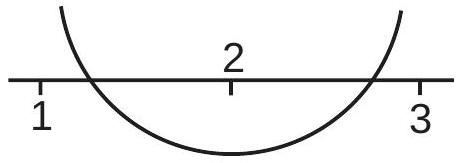
\includegraphics[max width=\textwidth, center]{2025_10_03_6412320a6c06d36206b5g-03}

\[
\begin{array}{ll}
f(1) \cdot f(2)<0 & \& f(2) \cdot f(3)<0 \\
(k-6)(k-8)<0 & \&(k-8)(k-6)<0 \\
k \in(6,8) & k \in(6,8)
\end{array}
\]

integral value of \(\mathrm{k}=7\)\\
68. Let \(\mathrm{f}: \mathrm{R}-\{0,1\} \rightarrow \mathrm{R}\) be a function such that \(f(x)+f\left(\frac{1}{1-x}\right)=1+x\). Then \(f(2)\) is equal to \(:\)\\
(1) \(\frac{9}{2}\)\\
(2) \(\frac{9}{4}\)\\
(3) \(\frac{7}{4}\)\\
(4) \(\frac{7}{3}\)

\section*{Official Ans. by NTA (2)}
Allen Ans. (2)\\
Sol. \(f(x)+f\left(\frac{1}{1-x}\right)=1+x\)

\[
x=2 \Rightarrow f(2)+f(-1)=3
\]

\[
x=-1 \Rightarrow f(-1)+f\left(\frac{1}{2}\right)=0
\]

\[
x=\frac{1}{2} \Rightarrow f\left(\frac{1}{2}\right)+f(2)=\frac{3}{2}
\]

\((1)+(3)-(2) \Rightarrow 2 f(2)=\frac{9}{2}\)\\
\(\therefore \mathrm{f}(2)=\frac{9}{4}\)\\
69. Let the plane \(P\) pass through the intersection of the planes \(2 x+3 y-z=2\) and \(x+2 y+3 z=6\), and be perpendicular to the plane \(2 x+y-z+1=0\). If \(d\) is the distance of P from the point \((-7,1,1)\), then \(\mathrm{d}^{2}\) is equal to:\\
(1) \(\frac{250}{83}\)\\
(2) \(\frac{15}{53}\)\\
(3) \(\frac{25}{83}\)\\
(4) \(\frac{250}{82}\)

Official Ans. by NTA (1)\\
Allen Ans. (1)\\
Sol. \(\mathrm{P} \equiv \mathrm{P}_{1}+\lambda \mathrm{P}_{2}=0\)\\
\((2+\lambda) x+(3+2 \lambda) y+(3 \lambda-1) z-2-6 \lambda=0\)\\
Plane P is perpendicular to \(\mathrm{P}_{3} \therefore \overrightarrow{\mathrm{n}} \cdot \overrightarrow{\mathrm{n}}_{3}=0\)\\
\(2(\lambda+2)+(2 \lambda+3)-(3 \lambda-1)=0\)\\
\(\lambda=-8\)\\
\(P \equiv-6 x-13 y-25 z+46=0\)\\
\(6 x+13 y+25 z-46=0\)\\
Dist from \((-7,1,1)\)\\
\(\mathrm{d}=\left|\frac{-42+13+25-46}{\sqrt{36+169+625}}\right|=\frac{50}{\sqrt{830}}\)\\
\(\mathrm{d}^{2}=\frac{50 \times 50}{830}=\frac{250}{83}\)\\
70. Let \(\mathrm{a}, \mathrm{b}\) be two real numbers such that \(\mathrm{ab}<0\). If the complex number \(\frac{1+a i}{b+i}\) is of unit modulus and \(\mathrm{a}+\mathrm{ib}\) lies on the circle \(|\mathrm{z}-1|=|2 \mathrm{z}|\), then a possible value of \(\frac{1+[a]}{4 b}\), where \([t]\) is greatest integer function, is :\\
(1) \(-\frac{1}{2}\)\\
(2) -1\\
(3) 1\\
(4) \(\frac{1}{2}\)

Official Ans. by NTA (1)\\
Allen Ans. (Bonus)

Sol. \(\quad a b<0\left|\frac{1+a i}{b+i}\right|=1\)\\
\(|1+\mathrm{ai}|=|\mathrm{b}+\mathrm{i}|\)\\
\(\mathrm{a}^{2}+1=\mathrm{b}^{2}+1 \Rightarrow \mathrm{a}= \pm \mathrm{b} \Rightarrow \mathrm{b}=-\mathrm{a} \quad\) as \(\mathrm{ab}<0\)\\
(a,b) lies on \(|z-1|=|2 z|\)\\
\(|\mathrm{a}+\mathrm{ib}-1|=2|\mathrm{a}+\mathrm{ib}|\)\\
\((a-1)^{2}+b^{2}=4\left(a^{2}+b^{2}\right)\)\\
\((a-1)^{2}=a^{2}=4\left(2 a^{2}\right)\)\\
\(1-2 \mathrm{a}=6 \mathrm{a}^{2} \Rightarrow 6 \mathrm{a}^{2}+2 \mathrm{a}-1=0\)\\
\(\mathrm{a}=\frac{-2 \pm \sqrt{28}}{12}=\frac{-1 \pm \sqrt{7}}{6}\)\\
\(\mathrm{a}=\frac{\sqrt{7}-1}{6} \& \mathrm{~b}=\frac{1-\sqrt{7}}{6}\)\\
\([\mathrm{a}]=0\)\\
\(\therefore \frac{1+[\mathrm{a}]}{4 \mathrm{~b}}=\frac{6}{4(1-\sqrt{7})}=-\left(\frac{1+\sqrt{7}}{4}\right)\)\\
or \([\mathrm{a}]=0\)\\
Similarly it is not matching with \(\mathrm{a}=\frac{-1-\sqrt{7}}{6}\)\\
No answer is matching.\\
71. The sum of the abosolute maximum and minimum values of the function \(\mathrm{f}(\mathrm{x})=\left|\mathrm{x}^{2}-5 \mathrm{x}+6\right|-3 \mathrm{x}+2\) in the interval \([-1,3]\) is equal to:\\
(1) 10\\
(2) 12\\
(3) 13\\
(4) 24

Official Ans. by NTA (1)\\
Allen Ans. (1)\\
Sol. \(f(x)=\left|x^{2}-5 x+6\right|-3 x+2\)\\
\(f(x)=\left\{\begin{array}{cc}x^{2}-8 x+8 & ; x \in[-1,2] \\ -x^{2}+2 x-4 & ; x \in[2,3]\end{array}\right.\)\\
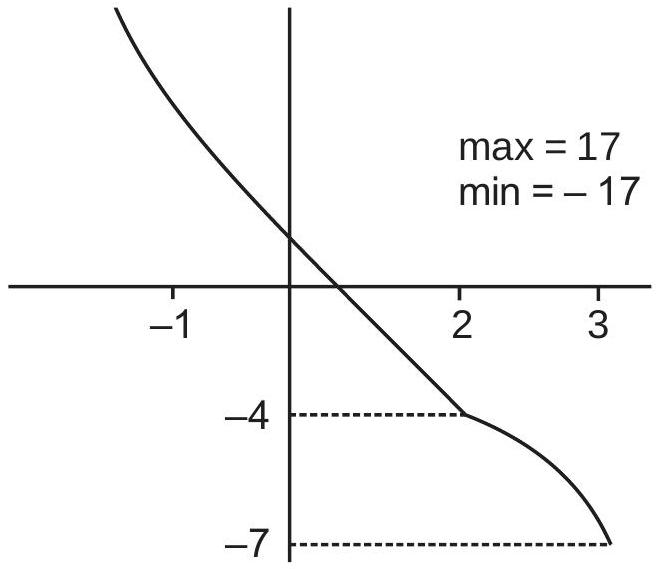
\includegraphics[max width=\textwidth, center]{2025_10_03_6412320a6c06d36206b5g-04(1)}\\
72. Let \(\mathrm{P}(\mathrm{S})\) denote the power set of \(\mathrm{S}=\{1,2,3, \ldots, 10\}\). Define the relations \(R_{1}\) and \(R_{2}\) on \(P(S)\) as \(A R_{1} B\) if \(\left(A \cap B^{c}\right) \cup\left(B \cap A^{c}\right)=\varnothing\) and \(A R_{2} B\) if \(A \cup B^{c}= \mathrm{B} \cup \mathrm{A}^{\mathrm{c}}, \forall \mathrm{A}, \mathrm{B} \in \mathrm{P}(\mathrm{S})\). Then :\\
(1) both \(R_{1}\) and \(R_{2}\) are equivalence relations\\
(2) only \(R_{1}\) is an equivalence relation\\
(3) only \(R_{2}\) is an equivalence relation\\
(4) both \(R_{1}\) and \(R_{2}\) are not equivalence relations

Official Ans. by NTA (1)\\
Allen Ans. (1)\\
Sol. \(\mathrm{S}=\{1,2,3, \ldots \ldots 10\}\)\\
\(\mathrm{P}(\mathrm{S})=\) power set of S\\
\(\mathrm{AR}, \mathrm{B} \Rightarrow(\mathrm{A} \cap \overrightarrow{\mathrm{B}}) \cup(\overrightarrow{\mathrm{A}} \cap \mathrm{B})=\phi\)\\
R1 is reflexive, symmetric\\
For transitive\\
\((\mathrm{A} \cap \overrightarrow{\mathrm{B}}) \cup(\overrightarrow{\mathrm{A}} \cap \mathrm{B})=\phi ;\{\mathrm{a}\}=\phi=\{\mathrm{b}\} \quad \mathrm{A}=\mathrm{B}\)\\
\((\mathrm{B} \cap \overrightarrow{\mathrm{C}}) \cup(\overrightarrow{\mathrm{B}} \cap \mathrm{C})=\phi \therefore \mathrm{B}=\mathrm{C}\)\\
\(\therefore \mathrm{A}=\mathrm{C}\) equivalence.\\
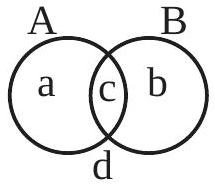
\includegraphics[max width=\textwidth, center]{2025_10_03_6412320a6c06d36206b5g-04}\\
\(\mathrm{R}_{2} \equiv \mathrm{~A} \cup \overrightarrow{\mathrm{~B}}=\overrightarrow{\mathrm{A}} \cup \mathrm{B}\)\\
\(\mathrm{R}_{2} \rightarrow\) Reflexive , symmetric\\
for transitive\\
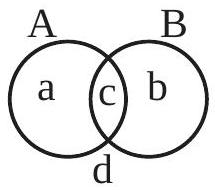
\includegraphics[max width=\textwidth, center]{2025_10_03_6412320a6c06d36206b5g-04(2)}\\
\(\mathrm{A} \cup \overrightarrow{\mathrm{B}}=\overrightarrow{\mathrm{A}} \cup \mathrm{B} \Rightarrow\{\mathrm{a}, \mathrm{c}, \mathrm{d}\}=\{\mathrm{b}, \mathrm{c}, \mathrm{d}\}\)\\
\(\{\mathrm{a}\}=\{\mathrm{b}\} \therefore \mathrm{A}=\mathrm{B}\)\\
\(\mathrm{B} \cup \overrightarrow{\mathrm{C}}=\overrightarrow{\mathrm{B}} \cup \mathrm{C} \Rightarrow \mathrm{B}=\mathrm{C}\)\\
\(\therefore \mathrm{A}=\mathrm{C} \quad \therefore \mathrm{A} \cup \overrightarrow{\mathrm{C}}=\overrightarrow{\mathrm{A}} \cup \mathrm{C} \quad \therefore\) Equivalence\\
73. The area of the region given by \(\left\{(\mathrm{x}, \mathrm{y}): \mathrm{xy} \leq 8,1, \leq \mathrm{y} \leq \mathrm{x}^{2}\right\}\) is :\\
(1) \(8 \log _{\mathrm{e}} 2-\frac{13}{3}\)\\
(2) \(16 \log _{e} 2-\frac{14}{3}\)\\
(3) \(8 \log _{\mathrm{e}} 2+\frac{7}{6}\)\\
(4) \(16 \log _{e} 2+\frac{7}{3}\)

Official Ans. by NTA (2)\\
Allen Ans. (2)

Sol.

\[
x y \leq 8 \quad 1 \leq y \leq x^{2}
\]

\begin{center}
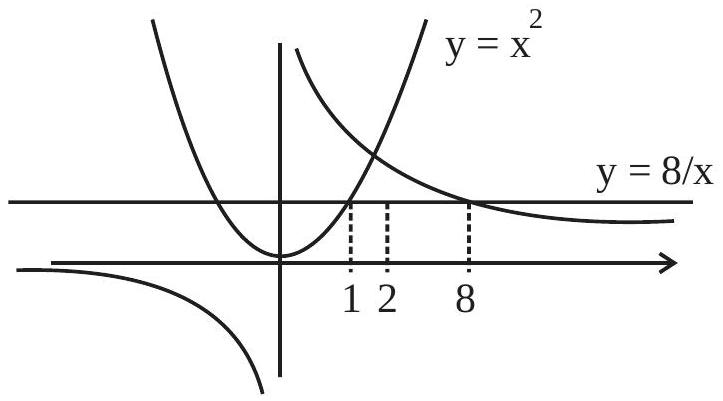
\includegraphics[max width=\textwidth]{2025_10_03_6412320a6c06d36206b5g-05}
\end{center}

Area \(=\int_{1}^{2}\left(x^{2}-1\right) d x+\int_{2}^{8}\left(\frac{8}{x}-1\right) d x\)\\
\(=\left(\frac{\mathrm{x}^{3}}{3}\right)_{1}^{2}+8(\ln \mathrm{x})_{2}^{8}-(\mathrm{x})_{1}^{8}\)\\
\(=\frac{7}{3}+8(2 \ell \mathrm{n} 2)-7\)\\
\(=16 \square \mathrm{n} 2-\frac{14}{3}\)\\
74. Let \(\alpha x=\exp \left(x^{\beta} y^{\gamma}\right)\) be the solution of the differential equation \(2 x^{2} y\) dy \(-\left(1-x y^{2}\right) d x=0\), \(x>0, y(2)=\sqrt{\log _{e} 2}\). Then \(\alpha+\beta-\gamma\) equals :\\
(1) 1\\
(2) -1\\
(3) 0\\
(4) 3

Official Ans. by NTA (1)\\
Allen Ans. (1)\\
Sol. \(\alpha \mathrm{x}=\mathrm{e}^{\mathrm{x}^{\beta} \cdot \mathrm{y}^{\gamma}}\)\\
\(2 x^{2} y \frac{d y}{d x}=1-x \cdot y^{2} \quad y^{2}=t\)\\
\(\mathrm{x}^{2} \frac{\mathrm{dt}}{\mathrm{dx}}=1-\mathrm{xt}\)\\
\(\frac{d t}{d x}+\frac{t}{x}=\frac{1}{x^{2}}\)\\
I.F. \(=\mathrm{e}^{\square \mathrm{nx}}=\mathrm{x}\)\\
\(\mathrm{t}(\mathrm{x})=\int \frac{1}{\mathrm{x}^{2}} \cdot \mathrm{x} d \mathrm{x}\)\\
\(\mathrm{y}^{2} . \mathrm{x}=\square \mathrm{nx}+\mathrm{C}\)\\
\(\therefore 2 . \square \mathrm{n} 2=\square \mathrm{n} 2+\mathrm{C}\)\\
\(\therefore \mathrm{C}=\square \mathrm{n} 2\)\\
Hence, \(\mathrm{xy}^{2}=\square \mathrm{n} 2 \mathrm{x}\)\\
\(\therefore 2 \mathrm{x}=\mathrm{e}^{\mathrm{x} \cdot \mathrm{y}^{2}}\)\\
Hence \(\alpha=2, \beta=1, \gamma=2\)\\
75. The value of the integral \(\int_{-\frac{\pi}{4}}^{\frac{\pi}{4}} \frac{x+\frac{\pi}{4}}{2-\cos 2 x} d x\) is :\\
(1) \(\frac{\pi^{2}}{6}\)\\
(2) \(\frac{\pi^{2}}{12 \sqrt{3}}\)\\
(3) \(\frac{\pi^{2}}{3 \sqrt{3}}\)\\
(4) \(\frac{\pi^{2}}{6 \sqrt{3}}\)

Official Ans. by NTA (4)\\
Allen Ans. (4)\\
Sol. \(\quad I=\int_{\frac{-\pi}{4}}^{\frac{\pi}{4}} \frac{x+\frac{\pi}{4}}{2-\cos 2 x} d x\)\\
\(\mathrm{x} \rightarrow-\mathrm{x}\)\\
\(I=\int_{\frac{-\pi}{4}}^{\frac{\pi}{4}} \frac{-x+\frac{\pi}{4}}{2-\cos 2 x} d x\)\\
(1) + (2)\\
\(2 \mathrm{I}=\int_{\frac{-\pi}{4}}^{\frac{\pi}{4}} \frac{\frac{\pi}{2}}{2-\cos 2 \mathrm{x}} \mathrm{dx}\)\\
\(\mathrm{I}=\frac{\pi}{4} \cdot 2 \int_{0}^{\frac{\pi}{4}} \frac{\mathrm{dx}}{2-\cos 2 \mathrm{x}} \mathrm{dx}\)\\
\(\mathrm{I}=\frac{\pi}{4} \cdot 2 \int_{0}^{\frac{\pi}{4}} \frac{\left(1+\tan ^{2} \mathrm{x}\right) \mathrm{dx}}{2\left(1+\tan ^{2} \mathrm{x}\right)-\left(1-\tan ^{2} \mathrm{x}\right)}\)\\
\(\mathrm{I}=\frac{\pi}{4} \int_{0}^{1} \frac{\mathrm{dt}}{3 \mathrm{t}^{2}+1}\)\\
\(\Rightarrow \mathrm{I}=\frac{\pi}{2 \sqrt{3}} \tan ^{-1} \sqrt{3}\)\\
\(\mathrm{I}=\frac{\pi^{2}}{6 \sqrt{3}}\)\\
76. Let \(9=\mathrm{x}_{1}<\mathrm{x}_{2}<\ldots<\mathrm{x}_{7}\) be in an A.P. with common difference d. If the standard deviation of \(\mathrm{x}_{1}, \mathrm{x}_{2} \ldots, \mathrm{x}_{7}\) is 4 and the mean is \(\overline{\mathrm{x}}\), then \(\overline{\mathrm{x}}+\mathrm{x}_{6}\) is equal to:\\
(1) \(18\left(1+\frac{1}{\sqrt{3}}\right)\)\\
(2) 34\\
(3) \(2\left(9+\frac{8}{\sqrt{7}}\right)\)\\
(4) 25

\section*{Official Ans. by NTA (2)}
\section*{Allen Ans. (2)}
Sol. \(\quad 9=\mathrm{x}_{1}<\mathrm{x}_{2}<\ldots \ldots .<\mathrm{x}_{7}\)\\
\(9,9+\mathrm{d}, 9+2 \mathrm{~d}, \ldots \ldots \ldots .9+6 \mathrm{~d}\)\\
0, d, 2d, ....... 6 d\\
\(\overline{\mathrm{x}}_{\text {new }}=\frac{21 \mathrm{~d}}{7}=3 \mathrm{~d}\)\\
\(16=\frac{1}{7}\left(0^{2}+1^{2}+\ldots \ldots .+6^{2}\right) \mathrm{d}^{2}-9 \mathrm{~d}^{2}\)\\
\(=\frac{1}{\not 7}\left(\frac{\not 6 \times \not 7 \times 13}{\not 6}\right) \mathrm{d}^{2}-9 \mathrm{~d}^{2}\)\\
\(16=4 \mathrm{~d}^{2}\)\\
\(\mathrm{d}^{2}=4\)\\
\(\mathrm{d}=2\)\\
\(\overline{\mathrm{x}}+\mathrm{x}_{6}=6+9+10+9\)\\
77. For the system of linear equations ax \(+\mathrm{y}+\mathrm{z}=1\), \(x+\) ay \(+z=1, x+y+a z=\beta\), which one of the following statements is NOT correct?\\
(1) It has infinitely many solutions if \(\alpha=2\) and \(\beta=-1\)\\
(2) It has no solution if \(\alpha=-2\) and \(\beta=1\)\\
(3) \(x+y+z=\frac{3}{4}\) if \(\alpha=2\) and \(\beta=1\)\\
(4) It has infinitely many solutions if \(\alpha=1\) and \(\beta=1\)

Official Ans. by NTA (1)\\
Allen Ans. (1)

Sol. \(\left|\begin{array}{lll}\alpha & 1 & 1 \\ 1 & \alpha & 1 \\ 1 & 1 & \alpha\end{array}\right|=0\)\\
\(\alpha\left(\alpha^{2}-1\right)-1(\alpha-1)+1(1-\alpha)=0\)\\
\(\alpha^{3}-3 \alpha+2=0\)\\
\(\alpha^{2}(\alpha-1)+\alpha(\alpha-1)-2(\alpha-1)=0\)\\
\((\alpha-1)\left(\alpha^{2}+\alpha-2\right)=0\)\\
\(\alpha=1, \alpha=-2,1\)\\
For \(\alpha=1, \beta=1\)\\
\(\left.\begin{array}{l}\mathrm{x}+\mathrm{y}+\mathrm{z}=1 \\ \mathrm{x}+\mathrm{y}+\mathrm{z}=\mathrm{b}\end{array}\right\}\) infinite solution\\
For \(\alpha=2, \beta=1\)\\
\(\Delta=4\)\\
\(\Delta_{1}=\left|\begin{array}{lll}1 & 1 & 1 \\ 1 & 2 & 1 \\ 1 & 1 & 2\end{array}\right|=3-1-1 \quad \Rightarrow \mathrm{x}=\frac{1}{4}\)\\
\(\Delta_{2}=\left|\begin{array}{lll}2 & 1 & 1 \\ 1 & 1 & 1 \\ 1 & 1 & 2\end{array}\right|=2-1=1 \quad \Rightarrow \mathrm{y}=\frac{1}{4}\)\\
\(\Delta_{3}=\left|\begin{array}{lll}2 & 1 & 1 \\ 1 & 2 & 1 \\ 1 & 1 & 1\end{array}\right|=2-1=1 \quad \Rightarrow \mathrm{z}=\frac{1}{4}\)\\
For \(\alpha=2 \Rightarrow\) unique solution\\
78. Let \(\vec{a}=5 \hat{i}-\hat{j}-3 \hat{k}\) and \(\vec{b}=\hat{i}+3 \hat{j}+5 \hat{k}\) be two vectors. Then which one of the following statements is TRUE?\\
(1) Projection of \(\vec{a}\) on \(\vec{b}\) is \(\frac{17}{\sqrt{35}}\) and the direction of the p\\
(2) Projection of \(\vec{a}\) on \(\vec{b}\) is \(\frac{-17}{\sqrt{35}}\) and the direction of the \(p\)\\
(3) Projection of \(\vec{a}\) on \(\vec{b}\) is \(\frac{17}{\sqrt{35}}\) and the direction of the projection vector is opposite to the direction of \(\vec{b}\)\\
(4) Projection of \(\vec{a}\) on \(\vec{b}\) is \(\frac{-17}{\sqrt{35}}\) and the direction of the projection vector is opposite to the direction of \(\vec{b}\)

Official Ans. by NTA (1)\\
Allen Ans. (Bonus)

Sol. \(\vec{a}=5 \hat{i}-\hat{j}-3 \hat{k}\)\\
\(\overrightarrow{\mathrm{b}}=\hat{\mathrm{i}}-3 \hat{\mathrm{j}}+5 \hat{\mathrm{k}}\)\\
\(\overrightarrow{\mathrm{a}} \cdot \hat{\mathrm{b}}=\frac{5-3-15}{\sqrt{35}}=-\frac{-13}{\sqrt{35}}\)\\
79. Let \(\mathrm{P}\left(\mathrm{x}_{0}, \mathrm{y}_{0}\right)\) be the point on the hyperbola \(3 \mathrm{x}^{2}- 4 y^{2}=36\), which is nearest to the line \(3 x+2 y=1\). Then \(\sqrt{2}\left(\mathrm{y}_{0}-\mathrm{x}_{0}\right)\) is equal to :\\
(1) -3\\
(2) 9\\
(3) -9\\
(4) 3

\section*{Official Ans. by NTA (3)}
Allen Ans. (3)\\
Sol. \(3 x^{2}-4 y^{2}=36 \quad 3 x+2 y=1\)\\
\(\mathrm{m}=-\frac{3}{2}\)\\
\(\mathrm{m}=+\frac{\sec \theta 3}{\sqrt{12} \cdot \tan \theta}\)\\
\(\Rightarrow \frac{3}{\sqrt{12}} \times \frac{1}{\sin \theta}=\frac{-3}{2}\)\\
\(\sin \theta=-\frac{1}{\sqrt{3}}\)\\
\((\sqrt{12} \cdot \sec \theta, 3 \tan \theta)\)\\
\(\left(\sqrt{12} \cdot \frac{\sqrt{3}}{\sqrt{2}},-3 \times \frac{1}{\sqrt{2}}\right) \Rightarrow\left(\frac{6}{\sqrt{2}}, \frac{-3}{\sqrt{2}}\right)\)\\
80. If \(y(x)=x^{x}, x>0\), then \(y^{\prime \prime}(2)-2 y^{\prime}(2)\) is equal to :\\
(1) \(8 \log _{\mathrm{e}} 2-2\)\\
(2) \(4 \log _{e} 2+2\)\\
(3) \(4\left(\log _{\mathrm{e}} 2\right)^{2}-2\)\\
(4) \(4\left(\log _{\mathrm{e}} 2\right)^{2}+2\)

Official Ans. by NTA (3)\\
Allen Ans. (3)

Sol. \(\mathrm{y}^{\prime}=\mathrm{x}^{\mathrm{x}}\)\\
\(\mathrm{y}^{\prime}=\mathrm{x}^{\mathrm{x}}(1+\square \mathrm{nx})\)\\
\(\mathrm{y}^{\prime \prime}=\mathrm{x}^{\mathrm{x}}(1+\square \mathrm{nx})^{2}+\mathrm{x}^{\mathrm{x}} \cdot \frac{1}{\mathrm{x}}\)\\
\(\mathrm{y}^{\prime \prime}(2)=4(1+\square \mathrm{n} 2)^{2}+2\)\\
\(\mathrm{y}^{\prime}(2)=4(1+\square \mathrm{n} 2)\)\\
\(\mathrm{y}^{\prime \prime}(2)-2 \mathrm{y}^{\prime}(2)=4(1+\square \mathrm{n} 2)^{2}+2-8(1+\square \mathrm{n} 2)\)\\
\(=4(1+\square \mathrm{n} 2)[1+\square \mathrm{n} 2-2]+2\)\\
\(\left.=4(\square \mathrm{n} 2)^{2}-1\right)+2\)\\
\(=4(\square \mathrm{n} 2)^{2}-2\)

\section*{SECTION-B}
\begin{enumerate}
  \setcounter{enumi}{80}
  \item The total number of six digit numbers, formed using the digits \(4,5,9\) only and divisible by 6 , is\\
\(\_\_\_\_\) .
\end{enumerate}

Official Ans. by NTA (81)\\
Allen Ans. (81)\\
Sol. Taking single digit \(\rightarrow 444444 \quad \frac{6!}{6!}=1\)\\
Taking two digit \(\rightarrow\)\\
\((4,5)\)\\
444555\\
\((4,9)\)\\
444999\\
\(\frac{5!}{3!2!}=10\)\\
\(\frac{5!}{3!2!}=10\)

Taking three digit\\
\(4,5,9,4,4,4 \Rightarrow \frac{5!}{3!}=20\)\\
\(4,5,9,5,5,5 \Rightarrow \frac{5!}{4!}=5\)\\
\(4,5,9,9,9,9 \Rightarrow \frac{5!}{4!}=5\)\\
\(4,5,9,4,5,9 \Rightarrow \frac{5!}{2!2!}=30\)\\
Total \(=81\)\\
82. Number of integral solutions to the equation \(\mathrm{x}+\mathrm{y}+\mathrm{z}=21\), where \(\mathrm{x} \geq 1, \mathrm{y} \geq 3, \mathrm{z} \geq 4\), is equal to\\
\(\_\_\_\_\) .

Official Ans. by NTA (105)

\section*{Allen Ans. (105)}
Sol. \(\quad{ }^{15} \mathrm{C}_{2}=\frac{15 \times 14}{2}=105\)\\
83. The line \(\mathrm{x}=8\) is the directrix of the ellipse \(\mathrm{E}: \frac{\mathrm{x}^{2}}{\mathrm{a}^{2}}+\frac{\mathrm{y}^{2}}{\mathrm{~b}^{2}}=1\) with the corresponding focus \((2,0)\). If the tangent to E at the point P in the first quadrant passes through the point \((0,4 \sqrt{3})\) and intersects the x -axis at Q , then \((3 \mathrm{PQ})^{2}\) is equal to\\
\(\_\_\_\_\) .

Official Ans. by NTA (39)\\
Allen Ans. (39)

\[
\begin{array}{ll}
\text { Sol. } & \frac{a}{e}=8 \ldots \ldots \ldots(1) \quad a e=2 \\
& 8 e=\frac{2}{e} \\
e^{2}=\frac{1}{4} \Rightarrow e=\frac{1}{2} \\
a=4 \\
b^{2}=a^{2}\left(1-e^{2}\right) \\
=16\left(\frac{3}{4}\right) \quad=12 \\
\frac{x \cos \theta}{4}+\frac{y \sin \theta}{2 \sqrt{3}}=1 \\
\sin \theta=\frac{1}{2} \\
\theta=30^{\circ} \\
P(2 \sqrt{3}, \sqrt{3}) \\
Q\left(\frac{8}{\sqrt{3}}, 0\right) \\
(3 P Q)^{2}=39
\end{array}
\]

\begin{enumerate}
  \setcounter{enumi}{83}
  \item If the x -intercept of a focal chord of the parabola \(y^{2}=8 x+4 y+4\) is 3 , then the length of this chord is equal to \(\_\_\_\_\) .\\
Official Ans. by NTA (16)
\end{enumerate}

Allen Ans. (16)\\
Sol.

\[
\begin{aligned}
& y^{2}=8 x+4 y+4 \\
& (y-2)^{2}=8(x+1) \\
& y^{2}=4 a x \\
& a=2, X=x+1, Y=y-2
\end{aligned}
\]

focus \((1,2)\)

\[
y-2=m(x-1)
\]

Put \((3,0)\) in the above line

\[
\mathrm{m}=-1
\]

Length of focal chord \(=16\)\\
85. If \(\int_{0}^{\pi} \frac{5^{\cos x}\left(1+\cos x \cos 3 x+\cos ^{2} x+\cos ^{3} x \cos 3 x\right) d x}{1+5^{\cos x}}=\frac{k \pi}{16}\), then k is equal to \(\_\_\_\_\) .

\section*{Official Ans. by NTA (26)}
\section*{Allen Ans. (13)}
\section*{Sol}
\(I=\int_{0}^{\pi} \frac{5^{\cos x}\left(1+\cos x \cos 3 x+\cos ^{2} x+\cos ^{3} x \cos 3 x\right)}{1+5^{\cos x}} d x\)\\
\(I=\int_{0}^{\pi} \frac{5^{-\cos x}\left(1+\cos x \cos 3 x+\cos ^{2} x+\cos ^{3} x \cos 3 x\right)}{1+5^{-\cos x}} d x\)\\
\(2 I=\int_{0}^{\pi}\left(1+\cos x \cos 3 x+\cos ^{2} x+\cos ^{3} x \cos 3 x\right) d x\)\\
\(\nsim I=\not 2 \int_{0}^{\frac{\pi}{2}}\left(1+\cos x \cos 3 x+\cos ^{2} x+\cos ^{3} x \cos 3 x\right) d x\)\\
\(I=\int_{0}^{\frac{\pi}{2}}\left(1+\sin x(-\sin 3 x)+\sin ^{2} x-\sin ^{3} x \sin 3 x\right) d x\)\\
\(2 I=\int_{0}^{\frac{\pi}{2}}\left(3+\cos 4 x+\cos ^{3} x \cos 3 x-\sin ^{3} x \sin 3 x\right) d x\)\\
\(2 I=\int_{0}^{\frac{\pi}{2}} 3+\cos 4 x+\left(\frac{\cos 3 x+3 \cos x}{4}\right) \cos 3 x-\sin 3 x\left(\frac{3 \sin x-\sin 3 x}{4}\right) d x\)

\[
2 I=\int_{0}^{\frac{\pi}{2}}\left(3+\cos 4 x+\frac{1}{4}+\frac{3}{4} \cos 4 x\right) d x
\]

\(2 \mathrm{I}=\frac{13}{4} \times \frac{\pi}{2}+\frac{7}{4}\left(\frac{\sin 4 \mathrm{x}}{4}\right)_{0}^{\frac{\pi}{2}} \Rightarrow \mathrm{I}=\frac{13 \pi}{16}\)\\
86. Let the sixth term in the binomial expansion of \(\left(\sqrt{2^{\log _{2}\left(10-3^{x}\right)}}+\sqrt[5]{2^{(x-2) \log _{2} 3}}\right)^{m}\), in the increasing powers of \(2^{(\mathrm{x}-2) \log _{2} 3}\), be 21 . If the binomial coefficients of the second, third and fourth terms in the expansion are respectively the first, third and fifth terms of an A.P., then the sum of the squares of all possible values of x is \(\_\_\_\_\) .

Official Ans. by NTA (4)\\
Allen Ans. (4)\\
Sol. \(\quad \mathrm{T}_{6}={ }^{\mathrm{m}} \mathrm{C}_{5}\left(10-3^{\mathrm{x}}\right)^{\frac{\mathrm{m}-5}{2}} \cdot\left(3^{\mathrm{x}-2}\right)=21\)\\
\({ }^{\mathrm{m}} \mathrm{C}_{1},{ }^{\mathrm{m}} \mathrm{C}_{2},{ }^{\mathrm{m}} \mathrm{C}_{3}\) are in A.P.\\
2. \({ }^{\mathrm{m}} \mathrm{C}_{2}={ }^{\mathrm{m}} \mathrm{C}_{1}+{ }^{\mathrm{m}} \mathrm{C}_{3}\)

Solving for m , we get\\
\(\mathrm{m}=2\) (rejected), 7\\
Put in equation (1)\\
\(21 .\left(10-3^{\mathrm{x}}\right) \frac{3^{\mathrm{x}}}{9}=21\)\\
\(3^{\mathrm{x}}=3^{0}, 3^{2}\)\\
\(\mathrm{x}=0,2\)\\
Sum of the squares of all possible values of \(x=4\)\\
87. If the term without \(x\) in the expansion of \(\left(x^{\frac{2}{3}}+\frac{\alpha}{x^{3}}\right)^{22}\) is 7315 , then \(|\alpha|\) is equal to \(\_\_\_\_\) .

Official Ans. by NTA (1)\\
Allen Ans. (1)\\
Sol. \(\quad \mathrm{T}_{\mathrm{r}+1}={ }^{22} \mathrm{C}_{\mathrm{r}} \cdot\left(\mathrm{x}^{\frac{2}{3}}\right)^{22-\mathrm{r}} \cdot(\alpha)^{\mathrm{r}}, \mathrm{x}^{-3 \mathrm{r}}\)\\
\(={ }^{22} \mathrm{C}_{\mathrm{r}} \cdot \mathrm{x}^{\frac{44}{3}-\frac{2 \mathrm{r}}{3}-3 \mathrm{r}}(\alpha)^{\mathrm{r}}\)\\
\(\frac{44}{3}=\frac{11 r}{3}\)\\
\(\mathrm{r}=4\)\\
\({ }^{22} \mathrm{C}_{4} \cdot \alpha^{4}=7315\)\\
\(\frac{22 \times 21 \times 20 \times 19}{24} . \alpha^{4}=7315\)\\
\(\alpha=1\)\\
88. The sum of the common terms of the following three arithmetic progressions.

3, 7, 11, 15, \(\_\_\_\_\) 399,

2, 5, 8, 11, \(\_\_\_\_\) 359 and

2, 7, 12, 17, \(\_\_\_\_\) 197, is equal to \(\_\_\_\_\) .

Official Ans. by NTA (321)\\
Allen Ans. (321)\\
Sol. 3, 7, 11, 15, \(\_\_\_\_\) 399\\
\(\mathrm{d}_{1}=4\)

2, 5, 8, 11, \(\_\_\_\_\) 359\\
\(\mathrm{d}_{2}=3\)

2, 7, 12, 17, \(\_\_\_\_\) 197\\
\(\mathrm{d}_{3}=5\)\\
\(\operatorname{LCM}\left(\mathrm{d}_{1}, \mathrm{~d}_{2}, \mathrm{~d}_{3}\right)=60\)\\
Common terms are 47, 107, 167\\
Sum \(=321\)\\
89. Let \(\alpha x+\beta y+y z=1\) be the equation of a plane passing through the point \((3,-2,5)\) and perpendicular to the line joining the points \((1,2,3)\) and \((-2,3,5)\). Then the value of \(\alpha \beta y\) is equal to\\
\(\_\_\_\_\) .

Official Ans. by NTA (6)\\
Allen Ans. (Bonus)\\
Sol. Given Equation is not equation of plane as yz is present. If we consider y is \(\gamma\) then answer would be 6 .

Normal vector of plane \(=3 \hat{\mathrm{i}}-\hat{\mathrm{j}}-2 \hat{\mathrm{k}}\)\\
Plane: \(3 \mathrm{x}-\mathrm{y}-2 \mathrm{z}+\lambda=0\)\\
Point \((3,-2,5)\) satisfies the plane\\
\(\lambda=-1\)\\
\(3 x-y-2 z=1\)\\
\(\alpha \beta y=6\)\\
90. The point of intersection \(C\) of the plane \(8 x+y+2 z=0\) and the line joining the points \(\mathrm{A}(-3,-6,1)\) and \(\mathrm{B}(2,4,-3)\) divides the line segment AB internally in the ratio \(\mathrm{k}: 1\). If \(\mathrm{a}, \mathrm{b}, \mathrm{c} (|a|,|b|,|c|\) are coprime \()\) are the direction ratios of the perpendicular from the point C on the line \(\frac{1-x}{1}=\frac{y+4}{2}=\frac{z+2}{3}\), then \(|a+b+c|\) is equal to\\
\(\_\_\_\_\) .

\section*{Official Ans. by NTA (10)}
Allen Ans. (10)\\
Sol. Plane : \(8 x+y+2 z=0\)\\
Given line \(\mathrm{AB}: \frac{\mathrm{x}-2}{5}=\frac{\mathrm{y}-4}{10}=\frac{\mathrm{z}+3}{-4}=\lambda\)\\
Any point on line ( \(5 \lambda+2,10 \lambda+4,-4 \lambda-3\) )\\
Point of intersection of line and plane\\
\(8(5 \lambda+2)+10 \lambda+4-8 \lambda-6=0\)\\
\(\lambda=-\frac{1}{3}\)\\
\(\mathrm{C}\left(\frac{1}{3}, \frac{2}{3},-\frac{5}{3}\right)\)\\
\(\mathrm{L}: \frac{\mathrm{x}-1}{-1}=\frac{\mathrm{y}+4}{2}=\frac{\mathrm{z}+2}{3}=\mu\)\\
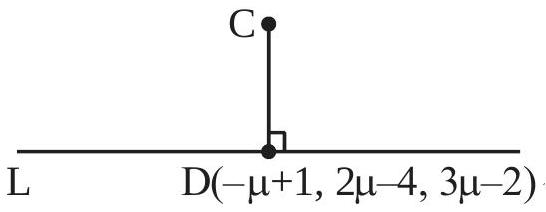
\includegraphics[max width=\textwidth, center]{2025_10_03_6412320a6c06d36206b5g-10}\\
\(\overrightarrow{\mathrm{CD}}=\left(-\mu+\frac{2}{3}\right) \hat{\mathrm{i}}+\left(2 \mu-\frac{14}{3}\right) \hat{\mathrm{j}}+\left(3 \mu-\frac{1}{3}\right) \hat{\mathrm{k}}\)\\
\(\left(-\mu+\frac{2}{3}\right)(-1)+\left(2 \mu-\frac{14}{3}\right) 2+\left(3 \mu-\frac{1}{3}\right) 3=0\)\\
\(\mu=\frac{11}{14}\)\\
\(\overrightarrow{\mathrm{CD}}=\frac{-5}{42}, \frac{-130}{42}, \frac{85}{42}\)\\
Direction ratios \(\rightarrow(-1,-26,17)\)\\
\(|\mathrm{a}+\mathrm{b}+\mathrm{c}|=10\)


\end{document}